\subsection{Simulated neutrino signal samples}\label{chap:montecarlo}

\begin{figure}[ht]
    \centering
    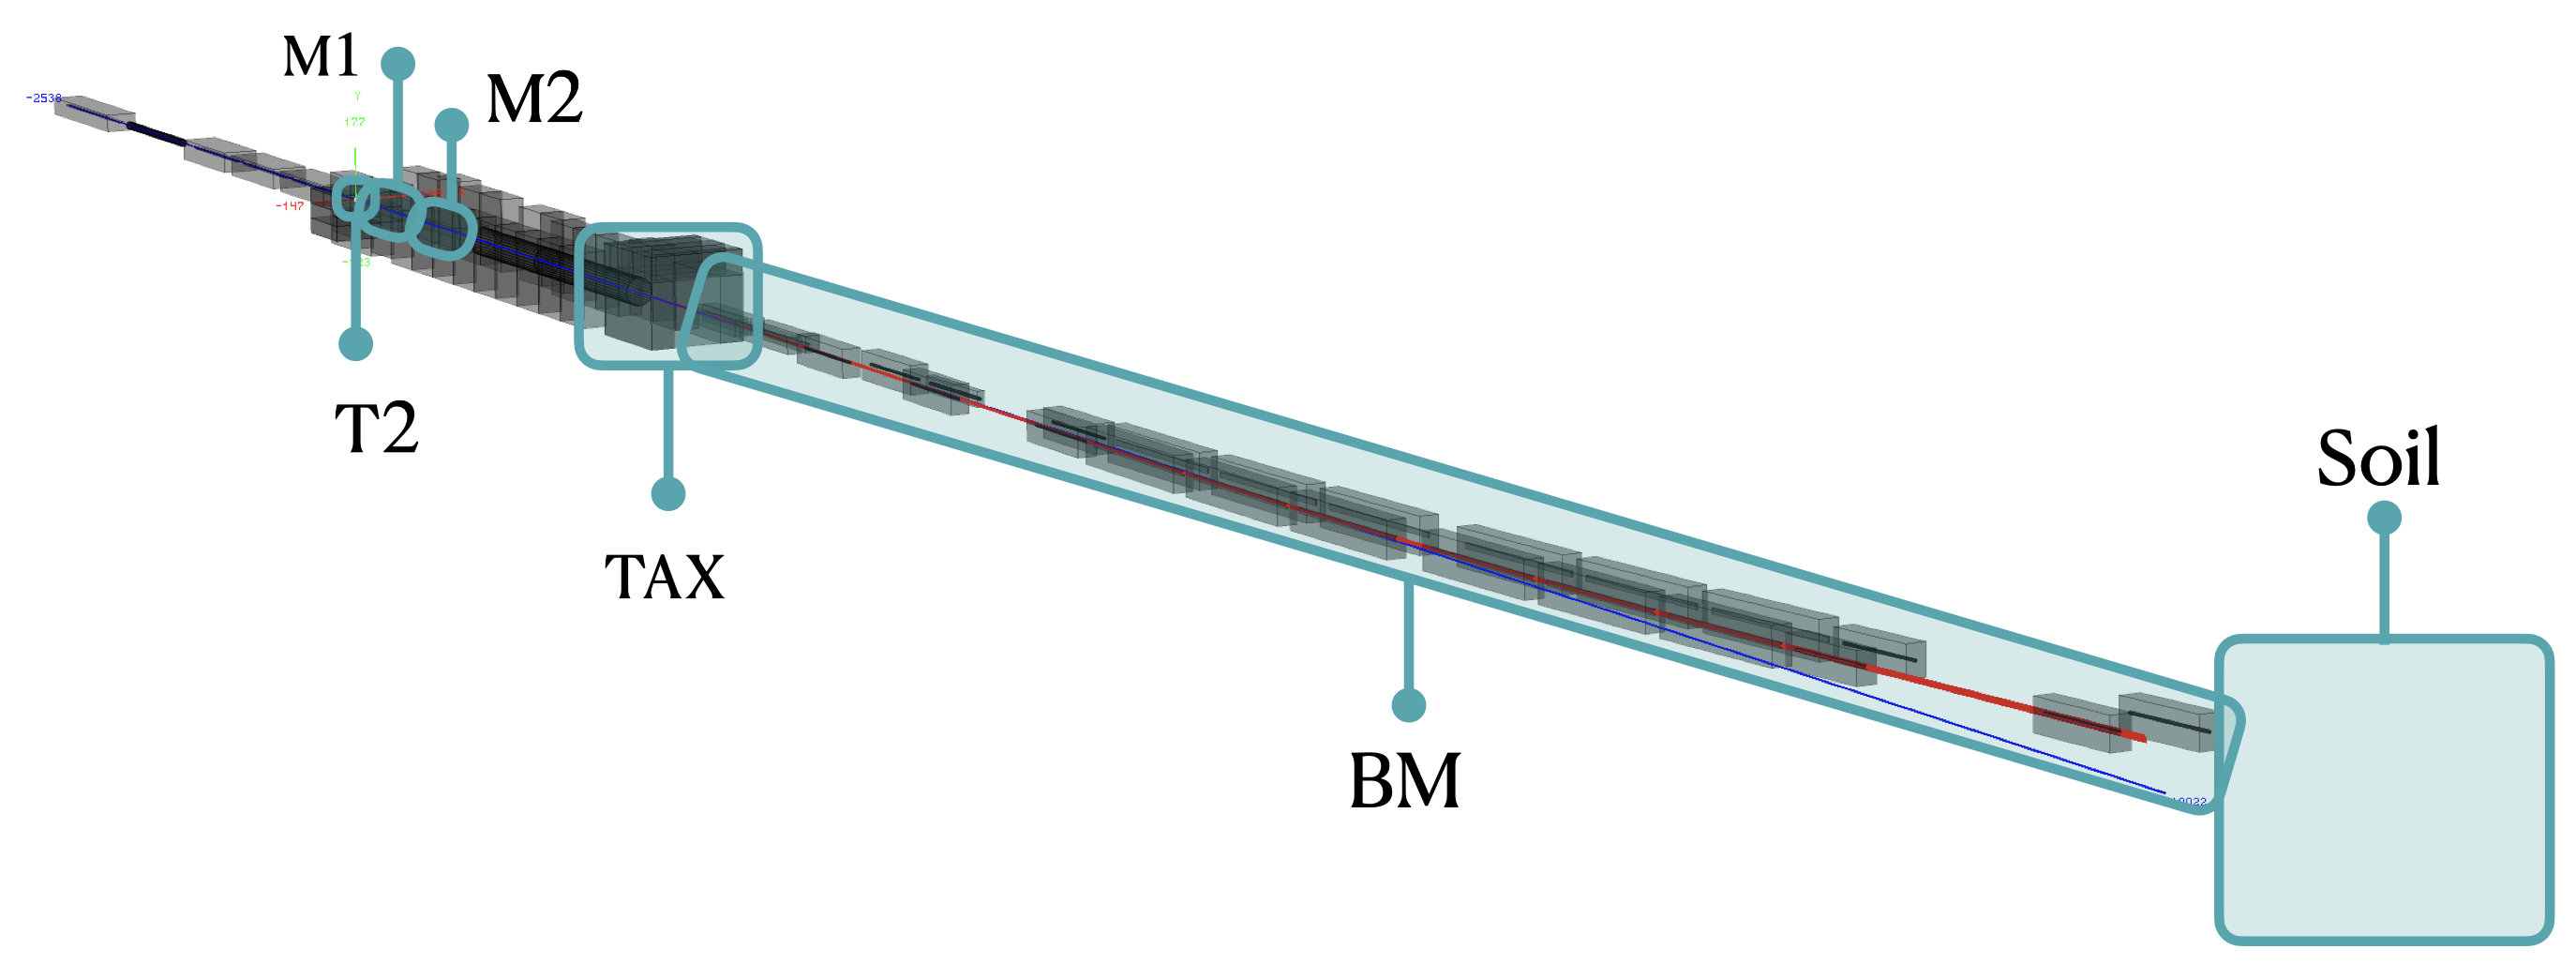
\includegraphics[width=1\linewidth]{sections/data_and_mc/plots/beam_geometry.png}
    \caption{Beam geometry included in the simulation to extract the spectra and the expected event rate. Only the first 100 m of the target location are simulated as after that there are 500 m of soil and all the building area of EHN1. T2 indicates the target and BM are beam magnets present after the target}
    \label{fig:geant4_geometry_beam}
\end{figure}

A Monte Carlo Geant4 simulation has been developed to predict the neutrino flux and energy spectra for different beam configurations, which form the signal sample considered in this study. The simulation starts from the SPS-extracted proton beam interacting with the target and includes all beamline elements within the first 100 m that constitute the target complex, as described in Section~\ref{sec:beam}. After this distance, the secondary beamlines continue above the T2 target height and there is then approximately 500~m of soil in front of the ProtoDUNE detectors. Only the first 100~m after the T2 target is simulated because this study focuses on the particles produced along the T2 target facility and few hadrons that could produce a neutrino or BSM particle incident on the ProtoDUNE detectors are expected to survive beyond this distance. Figure~\ref{fig:geant4_geometry_beam} illustrates the simulated beamline components. Simulating all the elements in the CERN North Area up to the Neutrino Platform would also add significant complexity to the flux simulation.
%After this distance, the beamlines continue in the upper part while at the target height there is 500 m of soil in front of ProtoDUNE detectors. As our focus are particles produced along T2 line and due to the complexity of including all elements located in the North Area building for all the lines, we only simulate that region.
%Following the collision of protons with the T2 target, the simulation encompasses all the magnets capable of deflecting the charged particles, the TAX, and the subsequent beamline extending to the soil.
%Figure~\ref{fig:geant4_geometry_beam} illustrates the simulated beamline components.

\begin{figure}[h!]
    \centering
    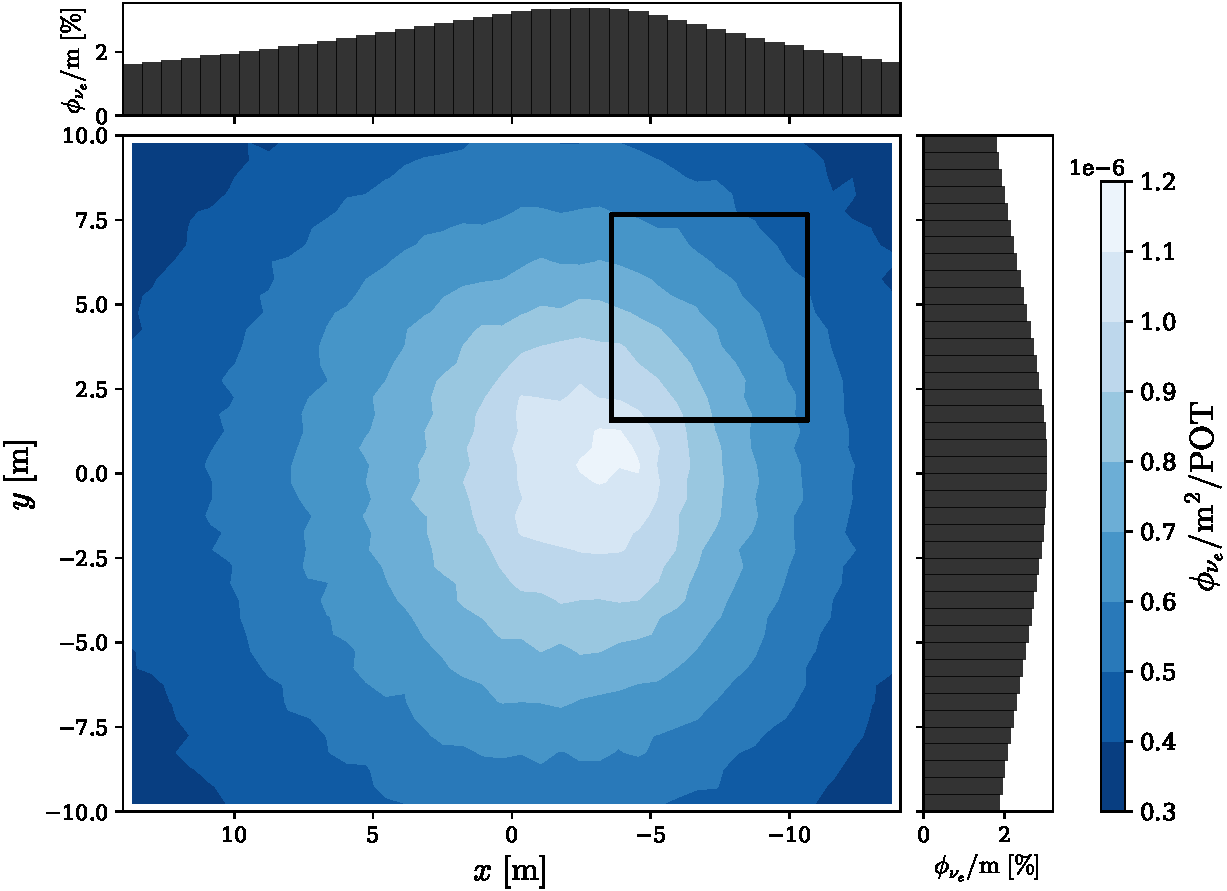
\includegraphics[width=0.49\linewidth]{sections/mc/plot/flux_np04_pos_nue.pdf}
    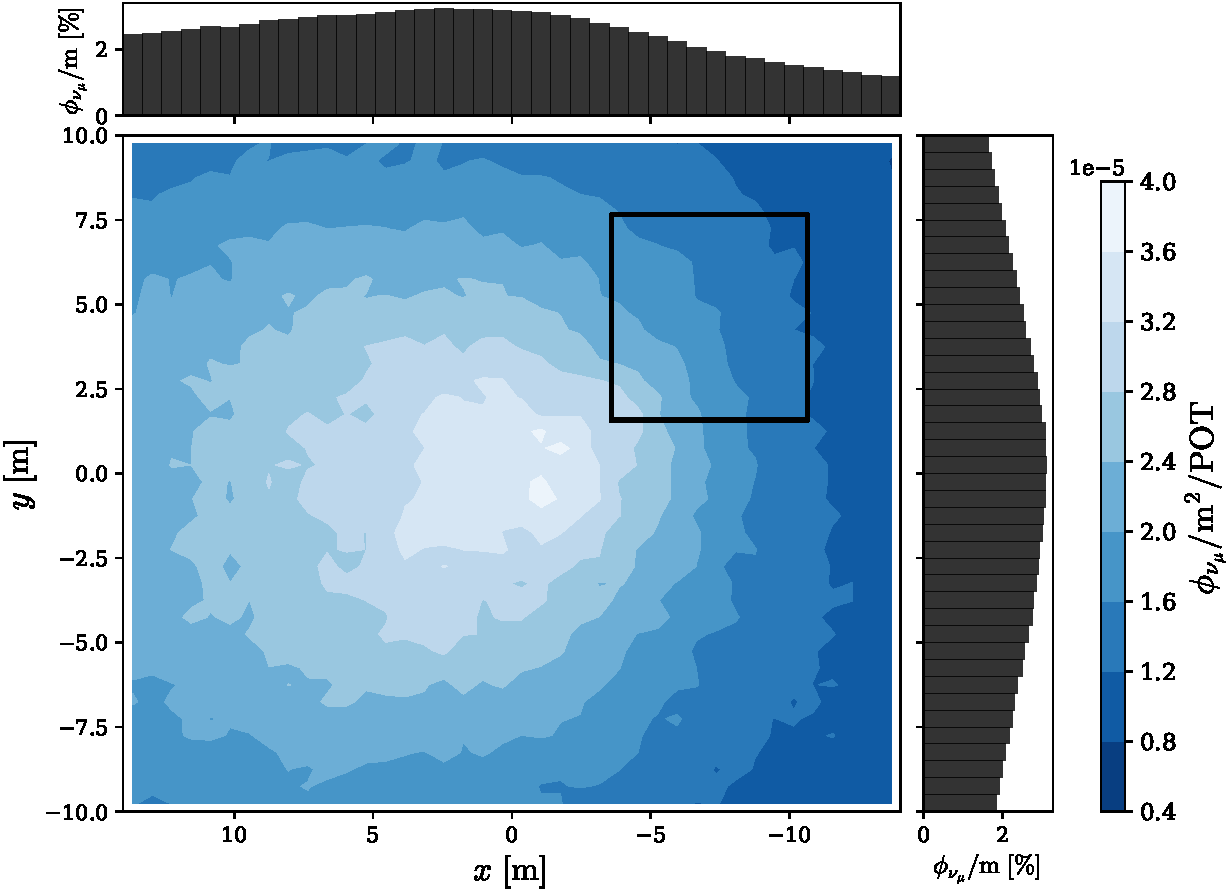
\includegraphics[width=0.49\linewidth]{sections/mc/plot/flux_np04_pos_numu.pdf}
    \caption{Simulated flux distribution of neutrino events in the XY-plane for $\nu_e$ (left) and $\nu_\mu$ (right) under the wNP04 configuration. The black square represents the projection of PD-HD. In contrast, the dashed box corresponds to the projection of the detector placed on the beam axis. Finally, the blue and yellow dots are the TPC center and DUNE reference point relative to the H4 beamline, respectively.}
    \label{fig:position_detector_josu}
\end{figure}

The positions of the ProtoDUNE detectors are not perfectly on axis with respect to the proton beam hitting the target. The neutrino flux at ProtoDUNE is evaluated using Monte Carlo simulation in which the geometrical acceptance of the detector is already incorporated into the event weights. This is shown in Figure \ref{fig:position_detector_josu} for the magnet configuration which maximizes the neutrinos flux (wNP04).

\begin{figure}[h!]
	\centering
    \begin{subfigure}{0.49\textwidth}
	   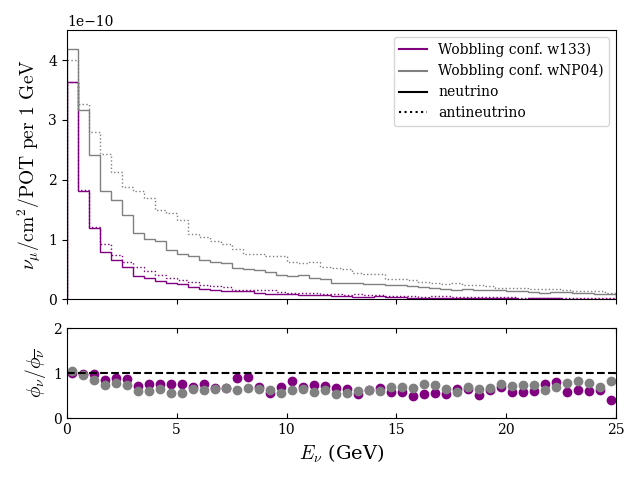
\includegraphics[width=0.99\columnwidth]{sections/mc/plot/numu_numubar_comparison_multimagconf_pdhd_flux_josu_new.png}
	   \caption{}
	   \label{fig:numu_numubar_fluxes}
    \end{subfigure}
    \hfill
    \begin{subfigure}{0.49\textwidth}
	   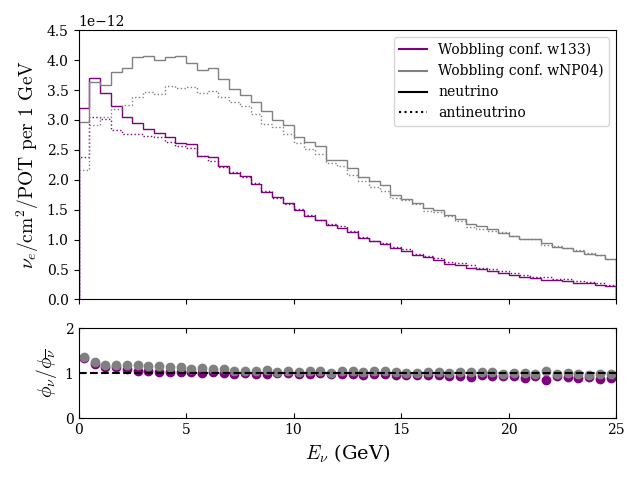
\includegraphics[width=0.99\columnwidth]{sections/mc/plot/nue_nuebar_comparison_multimagconf_pdhd_flux_josu_new.png}
	   \caption{}
	   \label{fig:nue_nuebar_fluxes}
    \end{subfigure}
    \caption{Simulated Neutrino fluxes for $\nu_{\mu}$ and $\bar{\nu}_{\mu}$ are shown in figure~\ref{fig:numu_numubar_fluxes} and fluxes for $\nu_{e}$ and $\bar{\nu}_{e}$ are shown in Figure~\ref{fig:nue_nuebar_fluxes}. Both figures show the flux for neutrinos and antineutrinos assuming two different magnet wobbling configurations w133 and wNP04.}
    %and w000, where w000 is the beam configuration with wobbling magnets off. Only the magnet configurations w133 and wNP04 are considered in this paper.
    \label{fig:fluxes_nu_nubar}
\end{figure}

The simulated neutrino flux spectra for the two most distinct magnet configurations are shown in Figure~\ref{fig:fluxes_nu_nubar}. As introduced previously, the different configurations deviate the charged pions and kaons produced after the proton interaction with the T2 target in different ways depending on the charge sign, leading to significant differences between the $\nu_{\mu}$ and $\bar{\nu}_{\mu}$ energy spectra. This is particularly evident for the wNP04 magnet configuration, as can be seen in Figure~\ref{fig:numu_numubar_fluxes}. In contrast, for electron neutrinos in the w133 configuration, the neutrino and antineutrino flux spectra are similar, as illustrated in Figure~\ref{fig:nue_nuebar_fluxes}. This similarity arises because the leading contribution comes from $K^0_L$ decay, with only a sub-leading contribution from $K^\pm$ that introduces a small correction at low energies. The percentage of expected neutrinos crossing the ProtoDUNE detector, broken down by neutrino species and parent meson, is listed for the w133 and wNP04 configurations in Tables~\ref{tab:light_nu_w133} and \ref{tab:light_nu_wnp04} respectively.

\begin{table}[h]
\centering
\begin{tabular}{|c|c|c|c|c|c|}
\hline
\multicolumn{6}{|c|}{Wobbling configuration w133 (contribution to flux \%)}\\
\hline
\hline
Parent & $\nu_e$ & $\overline{\nu}_e$ & $\nu_\mu$ & $\overline{\nu}_\mu$ & All \\
\hline
$\pi^+$ & $4.1 \cdot 10^{-3}$ & $0$ & $34.1$ & $0$ & $34.1$ \\ 
$\pi^-$ & $0$ & $5.2 \cdot 10^{-3}$ & $0$ & $43.0$ & $43.0$ \\ 
$K^0_S$ & $2.2 \cdot 10^{-1}$ & $2.2 \cdot 10^{-1}$ & $1.4 \cdot 10^{-1}$ & $1.4 \cdot 10^{-1}$ & $7.1 \cdot 10^{-1}$ \\ 
$K^0_L$ & $1.8$ & $1.8$ & $1.2$ & $1.2$ & $5.9$ \\ 
$K^+$ & $5.9 \cdot 10^{-1}$ & $0$ & $8.0$ & $0$ & $8.5$ \\ 
$K^-$ & $0$ & $5.4 \cdot 10^{-1}$ & $0$ & $7.2$ & $7.7$ \\ 
\hline
\end{tabular}
\caption{Percentage of neutrinos crossing PD-HD for each parent meson produced in the target, assuming the w133 wobbling configuration.}
\label{tab:light_nu_w133}
\end{table}

\begin{table}[h]
\centering
\begin{tabular}{|c|c|c|c|c|c|}
\hline
\multicolumn{6}{|c|}{Wobbling configuration wNP04}\\
\hline
\hline
Parent & $\nu_e$ & $\overline{\nu}_e$ & $\nu_\mu$ & $\overline{\nu}_\mu$ & All \\
\hline
$\pi^+$ & $3.8\cdot 10^{-3}$ & $0$ & $31.3$ & $0$ & $31.3$ \\ 
$\pi^-$ & 0 & $5.7\cdot 10^{-3}$ & $0$ & $47.1$ & $47.1$ \\ 
$K^0_S$ & $1.1\cdot 10^{-1}$ & $1.1 \cdot 10^{-1}$ & $7.1 \cdot 10^{-2}$ & $7.1 \cdot 10^{-2}$ & $3.7 \cdot 10^{-1}$ \\ 
$K^0_L$ & $8.6\cdot 10^{-1}$ & $8.6 \cdot 10^{-1}$ & $5.7 \cdot 10^{-1}$ & $5.7 \cdot 10^{-1}$ & $2.9$ \\ 
$K^+$ & $7.1\cdot 10^{-1}$ & $0$ & $9.4$ & $0$ & $10.1$ \\ 
$K^-$ & $0$ & $5.9\cdot 10^{-1}$ & $0$ & $7.7$ & $8.3$ \\ 
\hline
\end{tabular}
\caption{Percentage of neutrinos crossing the detector for each parent meson produced in the target, assuming the wNP04 wobbling configuration.}
\label{tab:light_nu_wnp04}
\end{table}


The simulation of neutrino interactions within ProtoDUNE was handled by \href{https://larsoft.org/}{LArSoft}, which provides a complete workflow for implementing a Monte Carlo event generator within a Geant4 simulation of the detector volume and simulating the detector response~\cite{LArSoft, Church:2013hea}. The neutrino fluxes described previously were converted into a format readable by LArSoft and fed into GENIE, which is a widely used event generator for simulating neutrino interactions on nuclear targets~\cite{GENIE}. Samples of 50,000 neutrino interactions within the active volume of PD-HD were simulated for each of the two magnet configurations considered: wNP04 and w133. The expected number of interactions in the active TPC during one week of SPS beam is broken down by neutrino flavor in Table~\ref{tab:number_events}. Tau neutrinos are excluded as they compose a relatively negligible proportion of the expected neutrino flux.

\begin{table}[]
    \centering
    \begin{tabular}{|c|c|c|}
        \hline
        \multicolumn{3}{|c|}{\textbf{Weekly interactions}} \\
        \hline
        Wobbling Configuration & \textbf{w133} & \textbf{wNP04} \\
        \hline
        $\nu_\mu$ & 641 & 3462 \\
        $\bar{\nu}_\mu$ & 431 & 2250 \\
        $\nu_e$ & 92 & 221 \\
        $\bar{\nu}_e$  & 43 & 101 \\
        \hline
        Total & \textbf{1207} & \textbf{6034} \\
        \hline
    \end{tabular}
    \caption{Total (CC+NC) expected number of neutrinos interacting in the active volume of PD-HD for each neutrino flavor assuming a flux arising from two magnet wobbling configurations: w133 and wNP04. The event rates are calculated from GENIE simulation of neutrino interactions and correspond to the event rate spectra shown in Figure~\ref{fig:genie_larsoft_eventrates}. The total event rate is also shown.}
    \label{tab:number_events}
\end{table}

Figure \ref{fig:genie_larsoft_eventrates} shows the event rate spectrum as a function of true neutrino energy for neutrinos interacting in the active TPC of PD-HD over one week of SPS beam. The total event rate is decomposed into the two neutrino flavors (and anti-neutrinos) considered (sub-Figures~\ref{fig:wnp04_flavor_event_rate} and \ref{fig:w133_flavor_event_rate}) and whether the interaction was charged current  (CC) or neutral current (NC) (sub-Figures~\ref{fig:wnp04_ccnc_event_rate} and \ref{fig:w133_ccnc_event_rate}). The energy spectrum for the event rate peaks at less than 10~GeV, although there is a long tail of neutrino interactions with high energies of tens of GeV. Finally the dominant component in expected neutrino interaction rate is $\nu_{\mu}$ CC, however there are still significant NC and antineutrino components.

\begin{figure}[h]
	\centering
    \begin{subfigure}{0.49\textwidth}
	   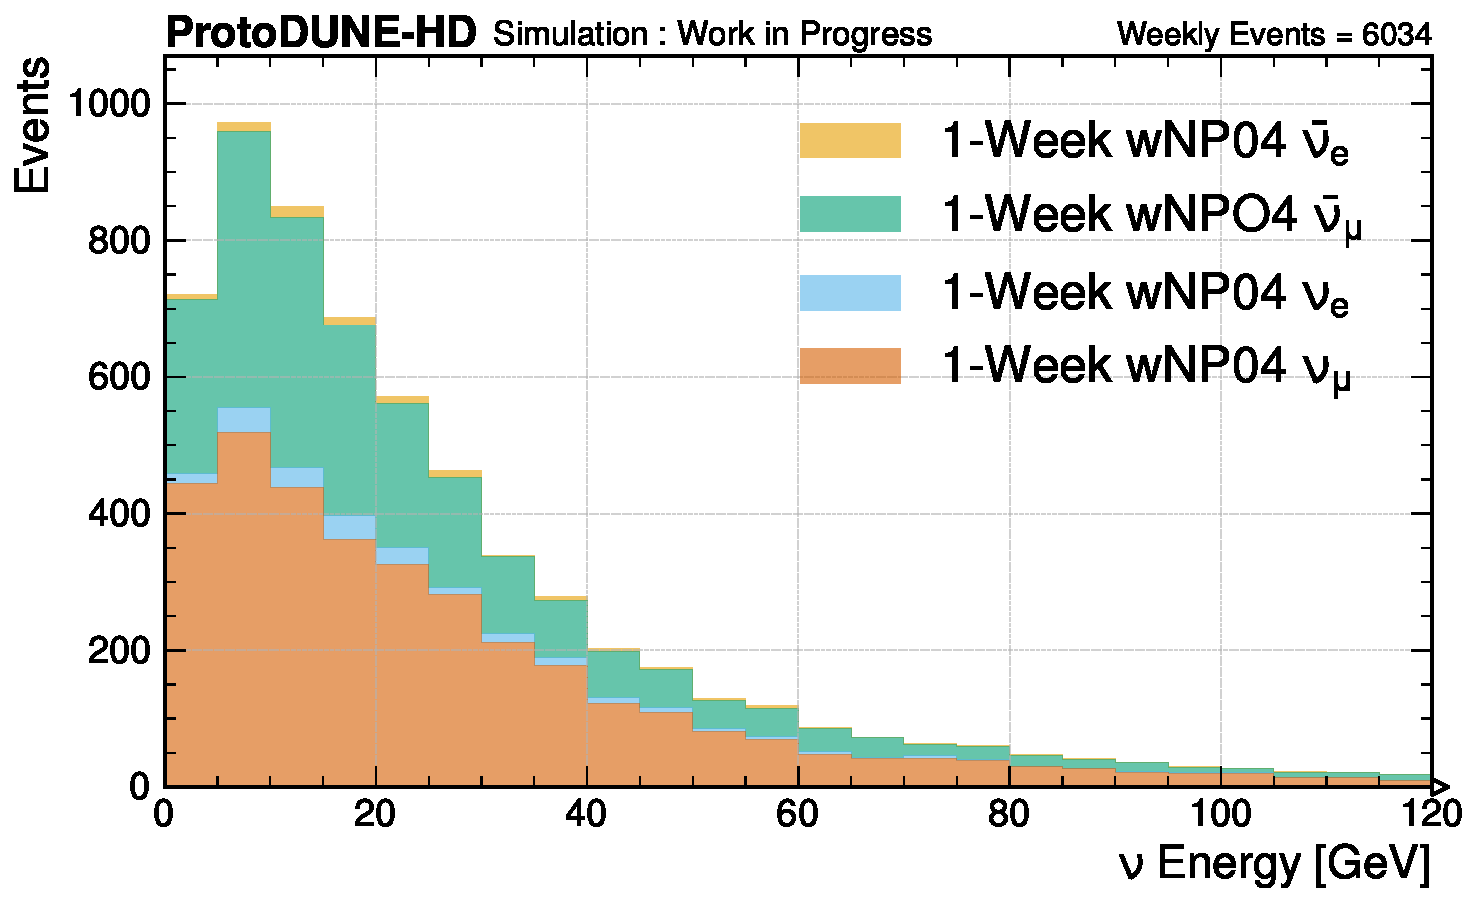
\includegraphics[width=0.99\columnwidth]{sections/mc/plot/nuE_wnp04_newleg_flav_sep_np04_stacked.pdf}
	   \caption{}
	   \label{fig:wnp04_flavor_event_rate}
    \end{subfigure}
    \hfill
    \begin{subfigure}{0.49\textwidth}
	   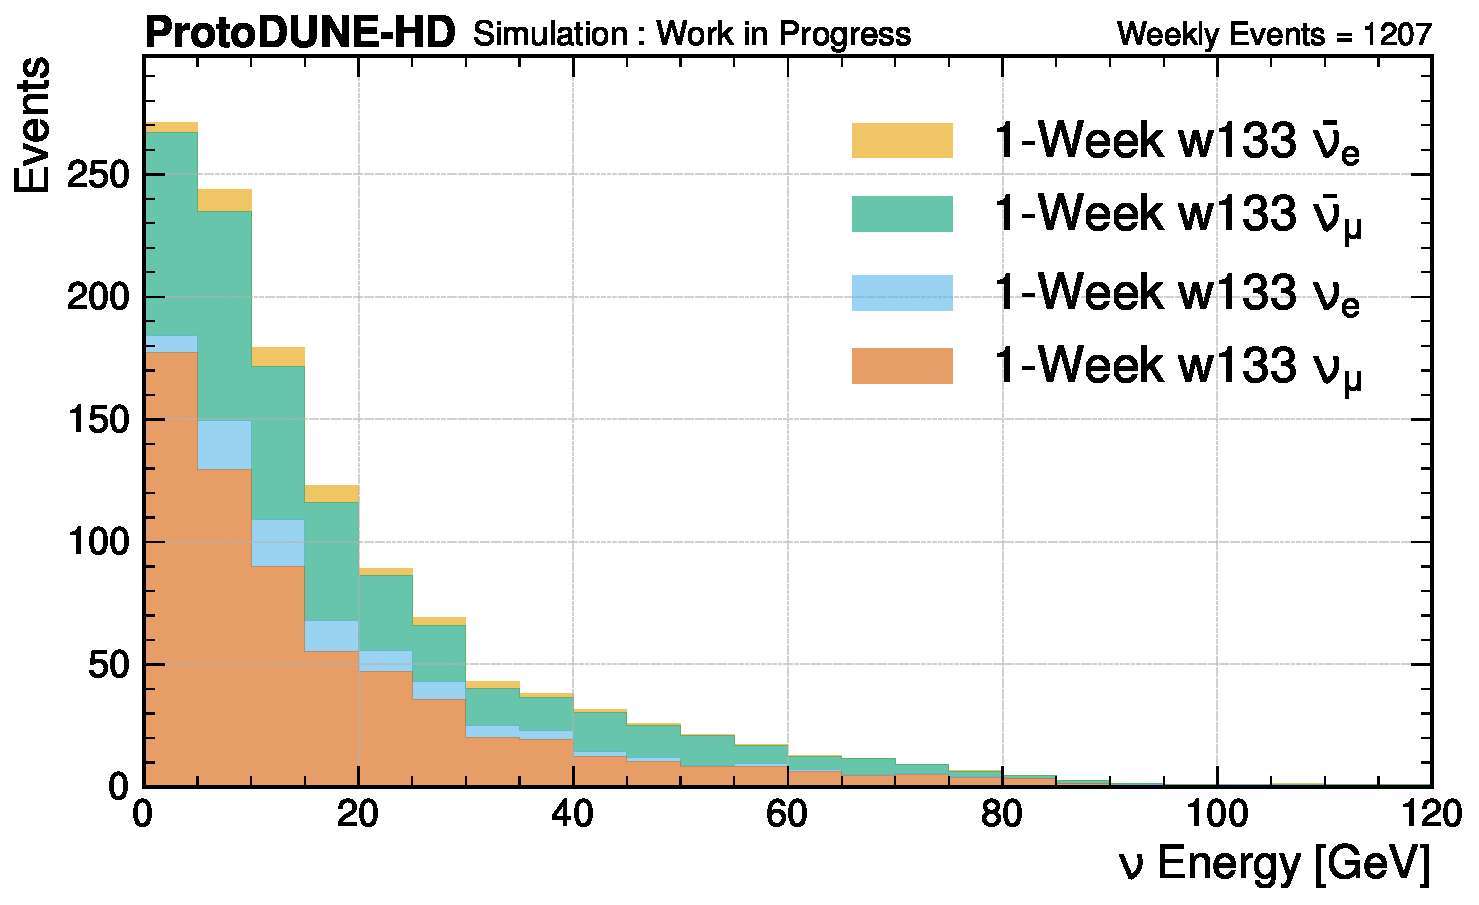
\includegraphics[width=0.99\columnwidth]{sections/mc/plot/nuE_w133_newleg_flav_sep_np04_stacked.pdf}
	   \caption{}
	   \label{fig:w133_flavor_event_rate}
    \end{subfigure}

    \begin{subfigure}{0.49\textwidth}
	   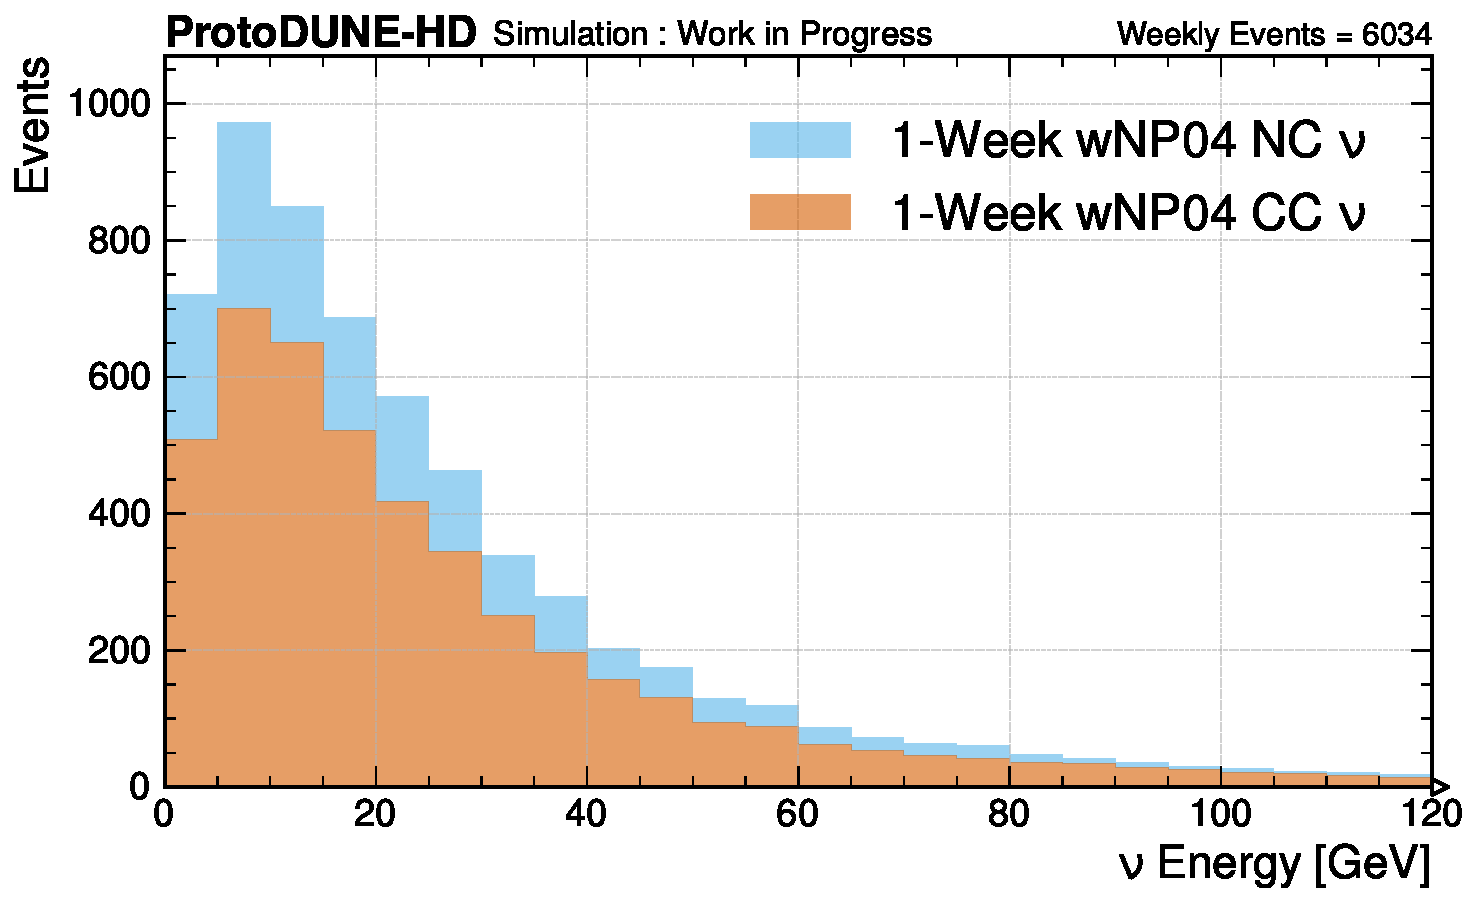
\includegraphics[width=0.99\columnwidth]{sections/mc/plot/nuE_wnp04_newleg_cc_nc_np04_stacked.pdf}
	   \caption{}
	   \label{fig:wnp04_ccnc_event_rate}
    \end{subfigure}
    \hfill
    \begin{subfigure}{0.49\textwidth}
	   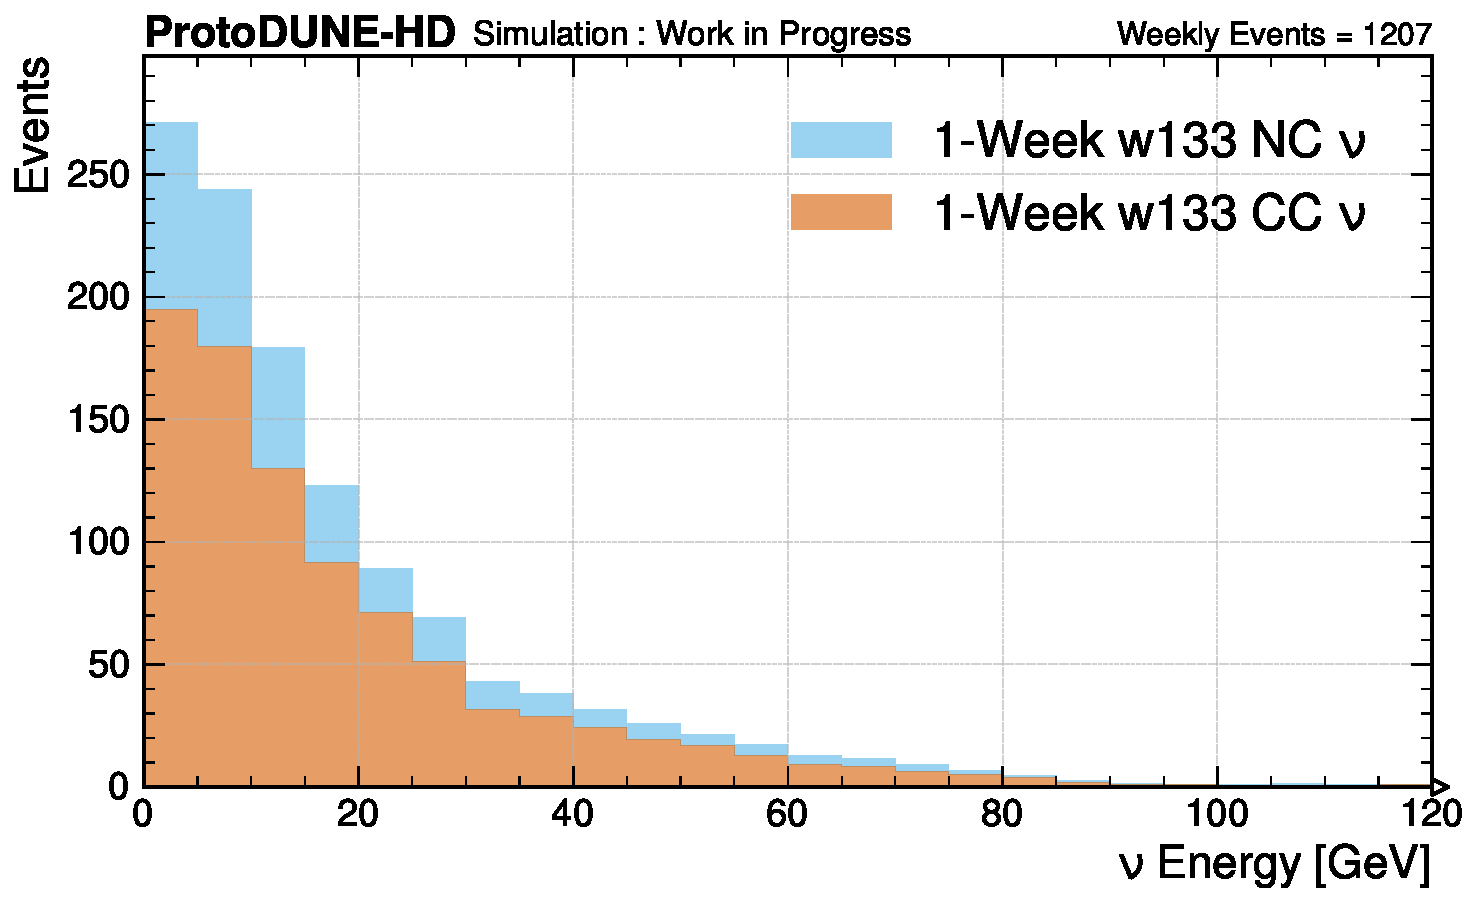
\includegraphics[width=0.99\columnwidth]{sections/mc/plot/nuE_w133_newleg_cc_nc_np04_stacked.pdf}
	   \caption{}
	   \label{fig:w133_ccnc_event_rate}
    \end{subfigure}
    \caption{Event rate predictions for one week of SPS beam as a function of true neutrino energy for two wobbling configurations: wNP04 (\ref{fig:wnp04_flavor_event_rate} and \ref{fig:wnp04_ccnc_event_rate}) and w133 (\ref{fig:w133_flavor_event_rate} and \ref{fig:w133_ccnc_event_rate}). The total event rates are a stacked combination of the contribution from each neutrino flavor or interaction type. Figures \ref{fig:wnp04_flavor_event_rate} and \ref{fig:w133_flavor_event_rate} show the breakdown of the total event rate by neutrino flavor. For both wobbling configurations, $\nu_{\mu}$ neutrinos are the largest component, although there is a significant contribution from $\bar{\nu}_{\mu}$. The relative contribution from CC versus NC neutrino interactions is shown in Figures \ref{fig:wnp04_ccnc_event_rate} and \ref{fig:w133_ccnc_event_rate}. The dominant interaction type is CC, however there is a large NC component as well.}
    \label{fig:genie_larsoft_eventrates}
\end{figure}

Once GENIE has generated the neutrino interaction within the detector, LArSoft runs several simulation stages. First, Geant4 simulates energy deposits within the detector volume. Then the detector response is simulated by generating the expected waveforms on the wire planes due to the Geant4 energy deposits. A hit-finding algorithm then generates reconstructed hits from the raw waveforms on each of the three wire planes. Finally, Pandora reconstruction clusters these hits together into reconstructed objects that can be used in the analysis described in Section~\ref{chap:Analyzer}~\cite{Pandora_2015}. A particular Pandora configuration is used that combines a reconstruction that identifies clear cosmic tracks to be removed and DUNE far detector neutrino reconstruction that searches for neutrino interaction vertices. 

The final simulated event rates are weighted in order to match the expected  exposure in units of protons-on-target (POT) for the data collected in a given run. To extract that number we use the CERN \href{http://timber.cern.ch}{TIMBER} application. It offers access to CERN Accelerator Logging Service data. From TIMBER, one extracts a time flag per spill, which indicates the beginning and end of the spill, as well as the POT. For this study, a spill with actual beam is considered when the PoT threshold is above $10^{12}$ and denoted as \textit{spill on}. If it is not the case the spill is considered empty, and classified as \textit{spill off}. Here, \textit{spill off} denotes the time between and during spills which have less than $10^{12}$ PoT. Each Monte Carlo event is weighted by
\begin{equation}
    w_{MC}= \frac{\text{POT}_{\text{data}}}{\text{POT}_{\text{MC}}},
\end{equation}
where ${\text{POT}_{\text{data}}}$ is the total POT collected during the run, and ${\text{POT}_{\text{MC}}}$ is the total POT simulated in the Monte Carlo. In Figure~\ref{fig:genie_larsoft_eventrates} this weighting is applied assuming one-week of SPS beam POT.

Neutrino flux and interaction predictions carry inherent uncertainties, as we are not able to measure the initial flux coming from the target. Flux modeling depends on hadron production, focusing, and decay, all of which are only partially constrained experimentally, while interaction generators such as GENIE rely on models of neutrino–nucleus scattering that have limitations, particularly regarding nuclear effects. As a result, absolute event rates and detailed spectral features are subject to systematic uncertainties, and simulation results are most reliable for relative comparisons rather than precise normalizations.

\subsection{Cosmic ray induced background samples}
The main background for the analysis is the cosmic particles that enter the detector and deposit an amount of energy comparable to the one expected from the very energetic neutrinos. The trigger excludes the vast majority of cosmic-ray events, thus leaving only the rarest, very energetic ones. Simulating such rare events using the Monte Carlo would be computationally expensive because it would require first simulating the entire spectrum and then selecting only the cosmic events that pass the trigger conditions in a subsequent stage. 
% To estimate the cosmic background, data collected during a period when the SPS beam was turned off was utilized, thereby eliminating all potential beam-related background and signal sources, and leaving only the cosmic events.
The cosmic ray background was estimated from data taken when the SPS beam was not active.

Since the flux of cosmic events is expected to be constant in time, all the backgrounds are reweighted only based on the active time:
\begin{equation}
    w_{bkg}=\frac{\text{Time}_{\text{ Spill On}}}{\text{Time}_{\text{ Bkg Run}}}
\end{equation}
where ${\text{Time}_{\text{ Spill On}}}$ is the effective time in the data when the beam spill was turned on and ${\text{Time}_{\text{ Bkg Run}}}$ is the duration of the run, used to extract the background events.

\subsection{Beam-related backgrounds}

Depending on the configuration of the wobbling magnets, the secondary particles produced after the target and being transported in H4, H2 and H6 secondary lines can vary significantly. The main effect at the ProtoDUNE location is the amount of muons traversing the detector. We refer to these muons as {\it halo muons}. The muons are primarily produced by the decay of pions and kaons with energies of the order of tens of GeV. Simulation studies performed for the ProtoDUNE Single-Phase technical design report (TDR), when the detector was exposed to the dedicated low-energy test beam, demonstrated that the most intense region of the muon halo passes through the upper part of the Jura side of the cryostat~\cite{DUNE_SP_2017}, indicated in Figure~\ref{fig:top_view_scheme}. This is also illustrated in Figure~\ref{fig:muonhalo}, which shows that the muon halo flux is concentrated in the top left part of the cryostat front face.

%Updated simulations of the beam-related backgrounds are not available to add an additional background sample for this analysis. However, the muon halo flux is expected to be the primary source of beam-related background and conclusions can be drawn from this previous muon halo study for the ProtoDUNE Single-Phase TDR. The muon halo would contribute to the background of a search for neutrinos originating from the T2 target by either a muon being misidentified as a neutrino interaction or a muon decaying in-flight to a neutrino that then interacts in the PD-HD active volume. If either of these cases are a large contribution to the background then there should be a significant increase in the measured event rate when the SPS beam is on relative to when the beam is off in the upper Jura-side of PD-HD where the muon halo flux is at its most intense. 

%Updated simulations of the beam-related backgrounds, specially pions and muons, are not available to add an additional background sample for this analysis. In addition, the effect of having different wobbling configurations has not been simulated for all cases. This fact combined different experiments using the H4 and H2 beamlines and therefore the elements along the line makes difficult to trace back all possible beam-related backgrounds. 
%However, the muon halo flux is expected to be the primary source of beam-related background and conclusions can be drawn from this previous muon halo study for the ProtoDUNE Single-Phase TDR. 
The muon halo would contribute to the background of a search for neutrinos originating from the T2 target in two ways: either through a muon being misidentified as a neutrino interaction, or through a muon decaying in flight and producing a neutrino that subsequently interacts within the ProtoDUNE active volume.

If either of these processes were a significant background contribution, one would expect a measurable increase in the event rate when the SPS beam is on compared to when the beam is off, particularly on the upper Jura-side of PD-HD where the muon-halo flux is highest. Another potential source of background is neutrinos produced from muon decays. However, these neutrinos are typically lower in energy than those originating from pion and kaon decays. As described in the next section, such events are largely suppressed by the trigger requirements, which select high-energy interactions. Nevertheless, possible neutrinos may arise from the decay of pions or kaons produced along the line.

Additional beam-related backgrounds may arise from high-energy neutrons. In liquid argon, these neutrons have a high probability of undergoing hadronic interactions, with an interaction length of roughly 0.9 m. Consequently, most neutrons interact before reaching the fiducial volume. For example, a multi-GeV neutron must travel about 1–2 meters to reach the FV, corresponding to a survival probability of roughly 10–30$\%$. Applying fiducial volume cuts therefore significantly suppresses these backgrounds, although a small fraction of neutrons could still penetrate without interacting inelastically.
%Additional beam-related backgrounds could arise from high-energy neutrons. However, high-energy neutrons have a strong hadronic interaction probability in liquid argon, with an interaction length of less than approximately one meter. Consequently, these events are effectively removed by applying fiducial volume cuts.
%It is possible that muons or neutrinos interacting in the soil, concrete and beamline facilities upstream of PD-HD could produce neutrons .... say something about neutrons here? It may need a particle gun simulation of neutrons to show that they tend to interact early in the volume if they are there

\begin{figure}[h!]
    \centering
    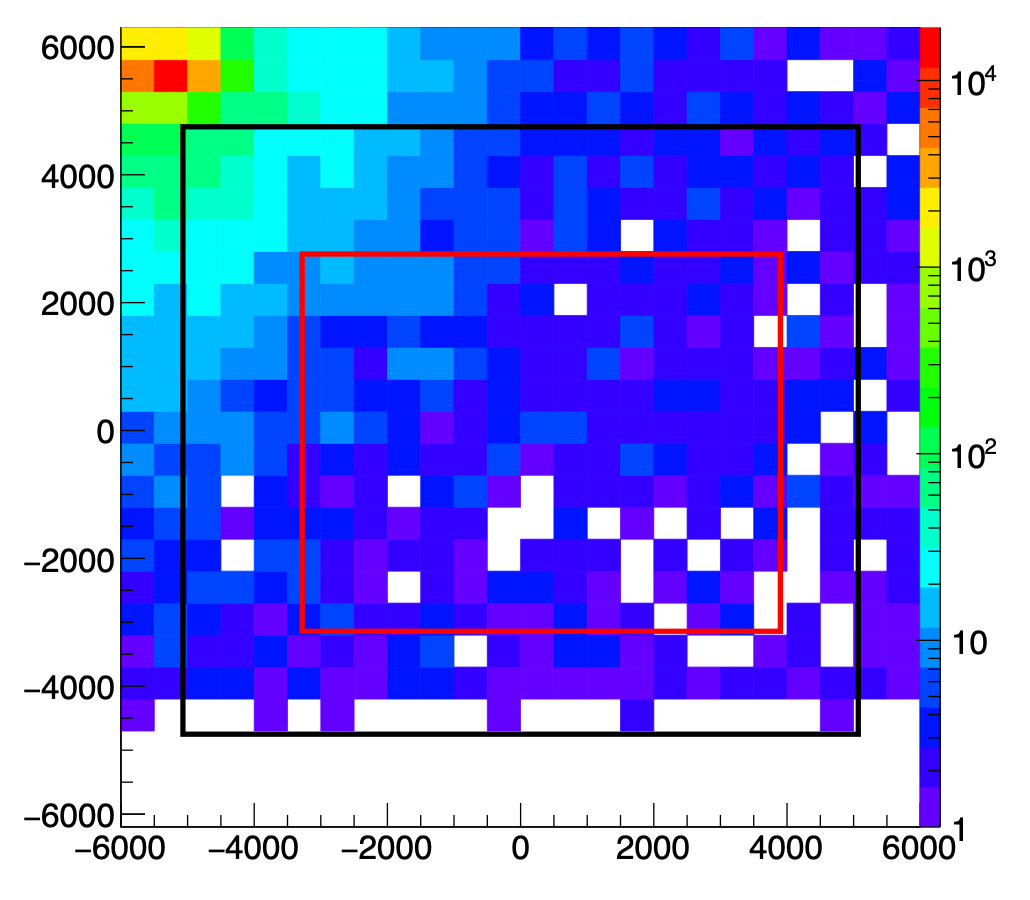
\includegraphics[width=0.8\linewidth]{sections/mc/plot/MuonHalo_xy_distribution_np04.png}
    \caption{Two-dimensional histogram showing the intensity of the muon halo flux intensity as a function of the ProtoDUNE x and y-coordinate given in millimeters, where the black and red boxes represent the front faces of the cryostat and active volume respectively. The x and y-axis are the x and y-coordinate of the PD-HD coordinate system and the color scale indicates the intensity of the muon halo flux. The definition of PD-HD coordinate system is given in Figure~\ref{fig:top_view_scheme}. This figure taken from ProtoDUNE-SP TDR~\cite{DUNE_SP_2017}.}
    \label{fig:muonhalo}
\end{figure}